\documentclass[12pt,a4paper,twosided]{article}

% Compile with "pandoc -S --template=design.template.tex design.md -o design.tex"
% Then add a:
% 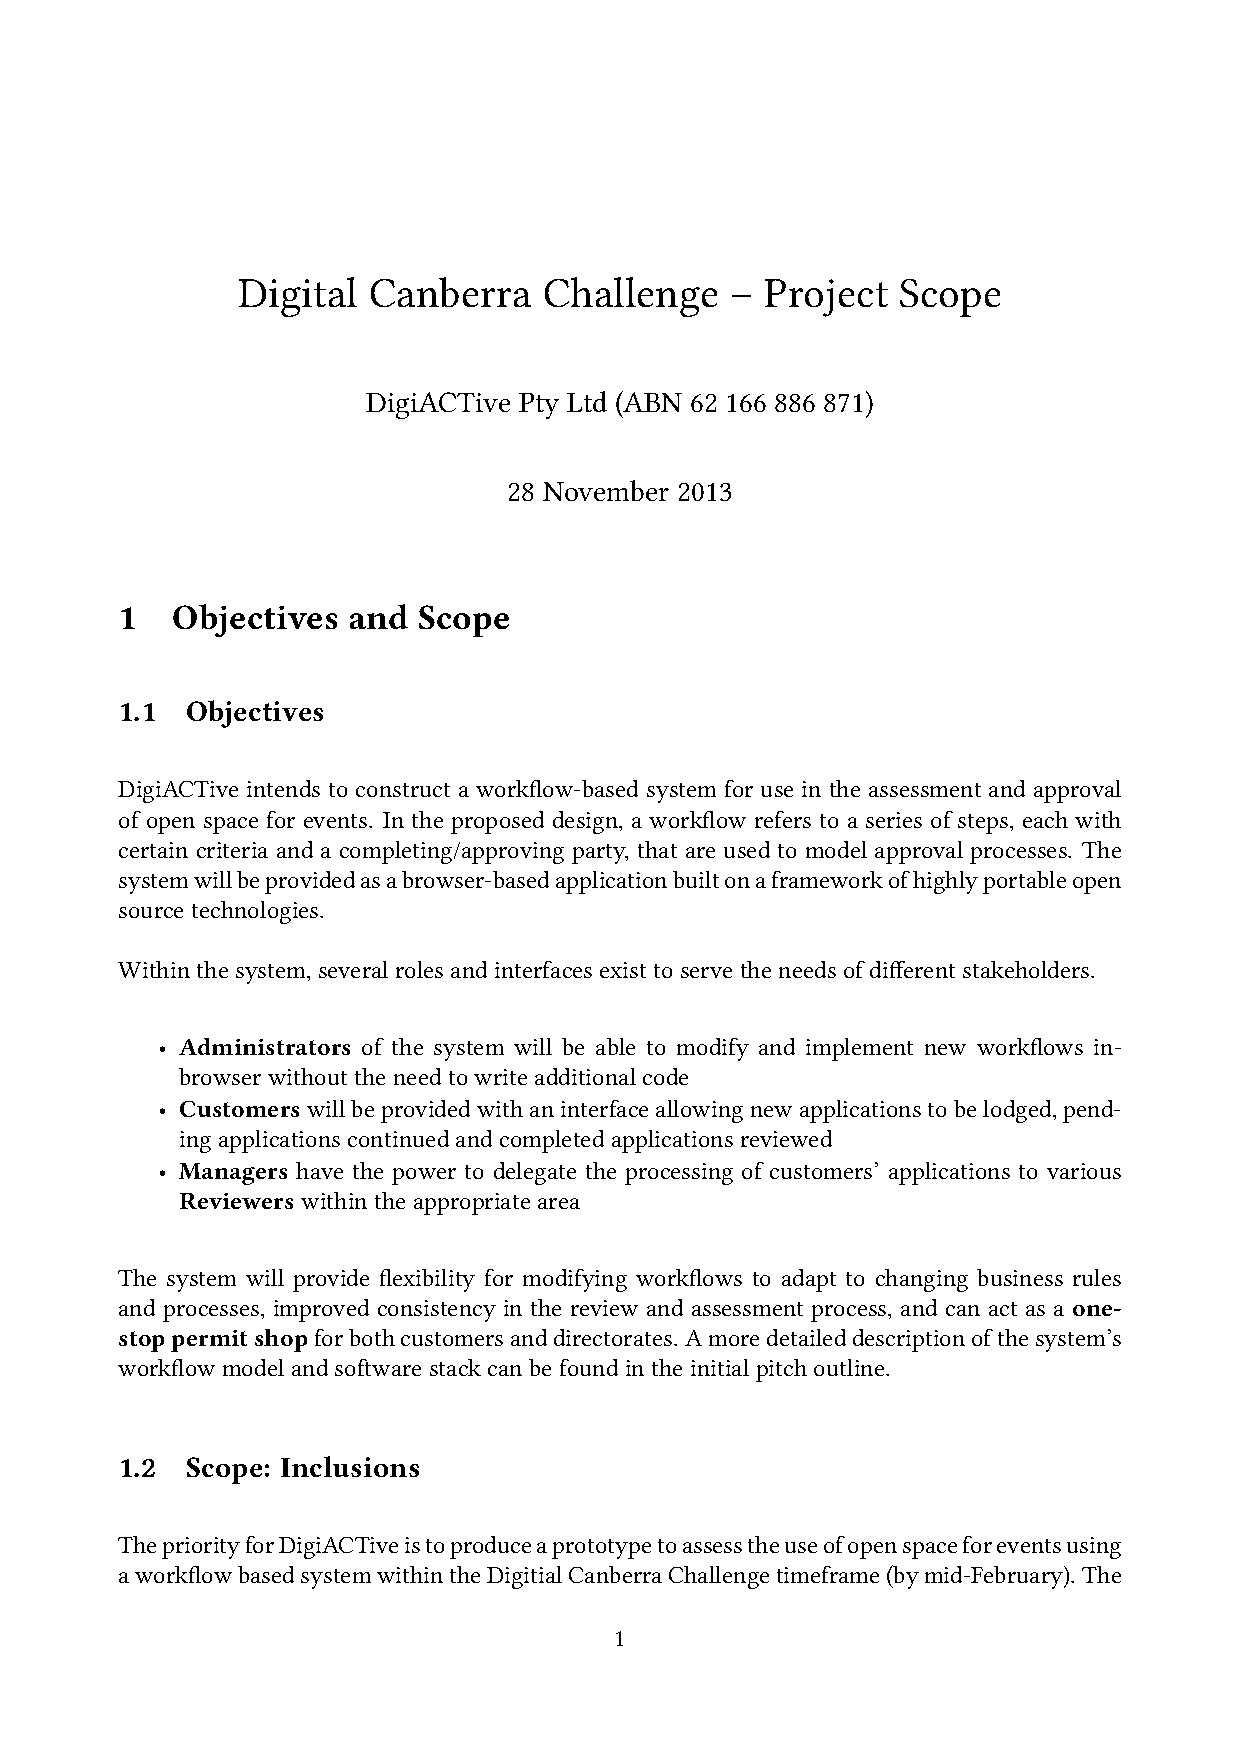
\includepdf[pages=1-6,nup=1x2,frame=true,landscape=true]{attached_work_scope.pdf}
% point, and remove the ?raw=true from the graphics, and add [width=0.9\textwidth]


\usepackage[utf8]{inputenc}
\usepackage{amsmath}
\usepackage{amsfonts}
\usepackage{amssymb}
\usepackage[top=3cm,bottom=3cm,left=2cm,right=2cm]{geometry}

\usepackage{setspace}
\setlength{\parindent}{0.0in}
\setlength{\parskip}{0.2in}

\usepackage{fancyhdr}
\setlength{\headheight}{15.2pt}
\chead{\sf DCC Project Plan \rm}
\pagestyle{fancy}




%\usepackage{times}
\usepackage[T1]{fontenc}
\usepackage{libertine}
\usepackage{graphicx}
\usepackage{pdfpages}
\usepackage{hyperref}
\renewcommand*\oldstylenums[1]{{\fontfamily{fxlj}\selectfont #1}}
\title{Digital Canberra Challenge -- Project Design}
\author{DigiACTive Pty Ltd (ABN 62 166 886 871)}
\date{16 December 2013}
\begin{document}
\maketitle
\begin{itemize}
\itemsep1pt\parskip0pt\parsep0pt
\item
  clarify ``As part of the application process\ldots{}'' (s16) - include
  example
\item
  clarify `Agencies that are out of the system' (s16) - I've added
  elsewhere that it's a web-based system. Fleur seems to be thinking
  that the system will be limited to within TAMS or might require
  locally installed software or something
\item
  change the example wireframe - applications that are part of/separate
  from application for public land permit. Also say `Assessment underway
  for liquor licence' (focus on the activity rather than the people
  involved\ldots{}) (s16.1.1)
\item
  `Use public land for an event' rather than `run an event'
\item
  ``How long the application has been pending'' - the clock resets when
  something's sent back for more documentation
\end{itemize}

More outstanding things + organisational accounts/sub-accounts to keep
organisational details consistent - associating events together
e.g.~Festival 2013 with Festival 2014 so that approvers can see past
event history (is this within scope for POC?) + a `traffic light' system
for different stages of the application (``How long the application has
been pending\ldots{}'')

\section{Background}

The ACT Government controls large portions of land within the ACT as
public unleased land, including many public parks and nature reserves
that are regularly used for events. Holding an event on public unleased
land generally requires approval. Parks and City Services handles
approximately 2,500 applications per year, covering a wide range of
events. Applications for large events can be highly complex, involving
approval from four or five other government agencies and many pages of
supporting documentation.

The current software used for handling land use approvals is basic and
provides only rudimentary features for managing the approval process --
it does not provide an end-to-end system to manage applications from
initial submission through to final approval. In particular, all
communication with applicants and with other agencies/stakeholders is
handled manually via email -- the officer handling the application must
manually update the database when an applicant submits an updated
document or another agency approves or rejects an application. This
process is time-consuming and error-prone.

The process of scoping the project also revealed the following pain
points that inform this project:

\begin{itemize}
\itemsep1pt\parskip0pt\parsep0pt
\item
  Approvals have to go through multiple agencies, which often fail to
  respond in a timely manner (if at all). The proliferation of contacts
  and lines of communication is difficult to manage.
\item
  It is unclear what approvals are needed to organise an event, leading
  to lots of unnecessary back-and-forth between the department and
  applicants.
\item
  Applicants are often unaware how long the process is likely to take,
  leading to disappointment when approvals are not ready in time.
\item
  Applicants are often unaware of the requirements of the different
  agencies, leading to lots of lengthy, time consuming and ultimately
  avoidable dialogs between parties.
\item
  Applicants are frustrated at how much work has to be done ``from
  scratch'' each time they organise an event.
\end{itemize}

\section{Objective}

The objective is two-fold:

\begin{itemize}
\itemsep1pt\parskip0pt\parsep0pt
\item
  To develop a proof of concept system to demonstrate a workflow-based,
  online system for use in the assessment and approval of open space for
  events.
\item
  To present a case study to the ACT Government and the eGov Cluster on
  the experience of the design and development.
\end{itemize}

\section{Outcomes}

\begin{itemize}
\itemsep1pt\parskip0pt\parsep0pt
\item
  To increase efficiency of government approval processes, especially
  multi-agency approvals
\item
  To improve the experience of those using the event approval system --
  in particular, to make it more obvious what is required of applicants
  and when, what the state of their applications are, and where to go
  for resources or for help
\item
  To allow TAMS to make an informed decision on proceeding with further
  development of a new approvals system
\end{itemize}

\section{Outputs}

There are two main outputs:

\begin{itemize}
\itemsep1pt\parskip0pt\parsep0pt
\item
  A proof of concept system for online assessment and approval of open
  space for events.
\item
  A case study documenting DigiACTive and TAMS' experience of the
  development process.
\end{itemize}

\section{Scope of Work/Assumptions and Constraints}

The project has been scoped in the attached scope document, which also
documents the assumptions and constraints.

\section{Governance and Reporting}

Per the project agreement, the project is guided by the Project Board.

The project board consists of:

\begin{itemize}
\itemsep1pt\parskip0pt\parsep0pt
\item
  \textbf{NICTA (eGov Cluster)}: Michael Phillips
\item
  \textbf{TAMS}: Rachel Reid
\item
  \textbf{DigiACTive}: Benjamin Roberts
\end{itemize}

Ongoing reporting occurs in the fortnightly project board meeting. The
case study is a summative/conclusory report.

\section{Schedule}

The project has a soft deadline of 26 Feb 2014 (end of last task on the
Gantt chart) and a hard deadline of 1 Mar 2014 (expiry of project
agreement).

The project is scheduled by the Gantt chart produced by TAMS and stored
on the eGovernment Cluster website.

\section{Budget}

The project budget is \$5,000, which is available to DigiACTive for
receipted expenses through the eGov Cluster.

\section{Stakeholders \& Communication Strategy}

\subsection{Collaborative Agreement Parties}

The Collaborative Agreement defines the interests and communication
strategy for \textbf{DigiACTive}, \textbf{the eGov Cluster} and
\textbf{TAMS}.

\subsection{Community Parties}

\begin{itemize}
\itemsep1pt\parskip0pt\parsep0pt
\item
  \textbf{MusicACT}

  \begin{itemize}
  \itemsep1pt\parskip0pt\parsep0pt
  \item
    \emph{Stakeholder interest}: MusicACT set the original challenge.
    Their interest is in the challenge POC being developed into a full
    system, thereby improving their experience in dealing with
    government whilst organising their events. They have identified a
    number of pain points which they would like to see improved. They
    see this project as part of a broader process of improving
    government services.
  \item
    \emph{Communication strategy}: DigiACTive has consulted them in the
    scoping process and will also work with them in the user testing
    part of the process.
  \end{itemize}
\item
  \textbf{Tuggeranong Community Festival}

  \begin{itemize}
  \itemsep1pt\parskip0pt\parsep0pt
  \item
    \emph{Stakeholder interest}: As the organisers of a large event in
    the territory they have an interest in the event organisation
    process being streamlined. They have highlighted a need for
    transparency and visibility regarding an applications processing
    status. They also identified a need for clarification of the
    relevant stakeholders requirements when issuing approvals.
  \item
    \emph{Communication strategy}: DigiACTive has consulted them in the
    scoping process and will also work with them in the user testing
    part of the process.
  \end{itemize}
\end{itemize}

\subsection{Other Affected Parties}

\begin{itemize}
\itemsep1pt\parskip0pt\parsep0pt
\item
  \textbf{SSICT}

  \begin{itemize}
  \itemsep1pt\parskip0pt\parsep0pt
  \item
    \emph{Stakeholder interest}: SSICT is responsible for the servers
    that the project would run on if the POC is converted to a full
    system. At this stage, none of the code is hosted on SSICT servers.
  \item
    \emph{Communication strategy}: SSICT's requirements are represented
    by their standards document. The solution is designed to comply with
    these standards. There is no ongoing communications planned with
    SSICT at this point.
  \end{itemize}
\item
  \textbf{Other Agencies}:

  \begin{itemize}
  \itemsep1pt\parskip0pt\parsep0pt
  \item
    \emph{Stakeholder Interest}: The approval process involves several
    government agencies, including the \textbf{National Capital
    Authority}, the \textbf{Emergency Services Agency}, the
    \textbf{Australian Federal Police}, the \textbf{ACT Insurance
    Authority}, \textbf{Roads ACT}, \textbf{ACT Heritage}, \textbf{TAMS
    Urban Treescapes Branch} and the \textbf{Environment Protection
    Authority}. Each agency is responsible for ensuring that
    applications meet the relevant requirements within the agency's
    areas of interest. Each agency has its own policies, procedures and
    systems for handling applications.
  \item
    \emph{Communication Strategy}: These agency's interests have been
    accounted for in the system design. Provision has been made for
    agencies to communicate effectively with TAMS staff and customers,
    whether they choose to adopt the system or remain with existing
    processes and systems (see the Technical Brief for more details).
    There is no ongoing communications planned with these agencies at
    this point.
  \end{itemize}
\end{itemize}

\section{Risk Management}

At this stage, the output is a proof of concept leading to an outcome of
informed decision making.

\subsection{Present Risks}

The risks to the initial outcome are limited:

\textbf{Risks:}

\begin{itemize}
\itemsep1pt\parskip0pt\parsep0pt
\item
  \textbf{Unexpected difficulty of technical component leading to
  unsatisfactory POC}

  \begin{itemize}
  \itemsep1pt\parskip0pt\parsep0pt
  \item
    \emph{Likelihood}: Very likely to occur at various points throughout
    project.
  \item
    \emph{Severity}: Potentially severe.
  \item
    \emph{Evaluation}: Requires action. See below.
  \end{itemize}
\item
  \textbf{Scope creep/change}

  \begin{itemize}
  \itemsep1pt\parskip0pt\parsep0pt
  \item
    This has been effectively mitigated by the signed scope document,
    and requires no further action.
  \end{itemize}
\item
  \textbf{Conflict in requirements/direction from stakeholders}

  \begin{itemize}
  \itemsep1pt\parskip0pt\parsep0pt
  \item
    TAMS/community groups pushing in different directions due to
    different foci, pain points.
  \item
    Ultimately this will be managed by the Project Board.
  \end{itemize}
\item
  \textbf{DigiACTive team newness/inexperience leading to poor
  performance}

  \begin{itemize}
  \itemsep1pt\parskip0pt\parsep0pt
  \item
    \emph{Likelihood}: Moderate.
  \item
    \emph{Severity}: Potentially severe.
  \item
    \emph{Evaluation}: Managed through the Digital Canberra
    Challenge/Collaborative Agreement governance structure.
  \end{itemize}
\end{itemize}

\subsubsection{Management Plan: unexpected technical difficulty}

It is virtually inevitable in a technical project that some aspect will
prove to be unexpectedly difficult.

A number of steps have been taken to reduce the likelihood of this
becoming a show-stopping issue:

\begin{itemize}
\itemsep1pt\parskip0pt\parsep0pt
\item
  The scope has been managed and restricted. In particular several
  systems that are unnecessary and difficult/time-consuming for a POC
  have been put out of the scope.
\item
  The project has been designed around well known and widely used tools
  that have proven to be flexible and scalable: we know the tools are up
  to the task.
\end{itemize}

We also have a number of strategies to allow us to manage any issues
that as they come up:

\begin{itemize}
\item
  The nature of the POC allows us to ``stub out'' functionality, to show
  how it would look and work without actually implementing it.

  For example, we have decided to ``stub out'' the payment system by
  assuming a transaction will succeed without completing further
  processing. This allows us to integrate payment steps into workflows,
  without spending our limited time implementing or integrating with a
  payment system.
\item
  Our regular meetings allow us to raise unexpected challenges,
  potentially finding novel ways around these problems that satisfy
  stakeholders' requirements in a way that is easier to implement.
\item
  Our links with the eGov Cluster, the innovation community in Canberra
  and with the ANU provide us with networks of experts that can help us
  resolve issues we may encounter.
\end{itemize}

Ultimately, this is an unavoidable risk that all software projects bear.
We are confident that our mitigation strategies are sufficient.

\subsubsection{Management Plan: DigiACTive team}

The DigiACTive team is new, and therefore has the usual risks of new
groups and companies.

The risks are largely mitigated by the structure of the Digital Canberra
Challenge and the governance arrangements from the Collaborative
Agreement.

\begin{itemize}
\itemsep1pt\parskip0pt\parsep0pt
\item
  The fortnightly meetings provide the \emph{accountability} necessary
  to detect problems early.
\item
  The involvement of the eGov Cluster and their experience with early
  stage commercialisation provides the \emph{resources} and
  \emph{networks} for DigiACTive to seek help correcting problems as
  they arise.
\item
  The structure of the challenge provides a definite end point where the
  project can be abandoned if it has become unfeasible.
\end{itemize}

\subsection{Avoided Risks/Out of Scope risks}

Risks will need to be reassessed should TAMS wish to proceed to a full
system after the proof of concept. However, as it stands, the project
poses low risk to TAMS:

\begin{itemize}
\itemsep1pt\parskip0pt\parsep0pt
\item
  \textbf{The output is a proof of concept that is not publicly
  accessible.} This closes off a large range of risks:

  \begin{itemize}
  \itemsep1pt\parskip0pt\parsep0pt
  \item
    No confidential user data can be lost or stolen as no confidential
    user data will enter the system.
  \item
    System malfunctions will not lead to embarrassment or public
    backlash as the system will not be open to the public.
  \item
    System malfunctions will not lead to downtime or lost productivity
    internally as the system will not be used beyond a small group of
    testers at this stage.
  \end{itemize}
\item
  TAMS is not committed to take the project further - if it is not fit
  for purpose or is going to be to expensive, TAMS can decide not to
  proceed with the project after the project agreement lapses on 1
  March. TAMS is not obligated to progress the project beyond that
  point.
\item
  The DCC budget is for expense reimbursement only, and is capped at
  \$5000. This is managed by the eGov Cluster.
\end{itemize}

\section{Related Projects}

The closest related work that DigiACTive is aware of is the existing
smart-form system. There is also an ongoing project within PACS to
develop a booking system for venue bookings.

Looking outside of PACS the other Digital Canberra Challenge project
presently running, regarding the booking of drivers' license tests, is
tangentially related in that it's a booking system, but targets a
different use case and proceeds from a much simpler model -- there is no
need for multi-agency involvement, for example.

\subsection{Future Extensions}

The project scope is explicitly restricted to a proof of concept. Should
the project proceed to a full system, there are a couple of related
projects:

\begin{itemize}
\itemsep1pt\parskip0pt\parsep0pt
\item
  \href{http://planyourpicnic.org.au}{Plan Your Picnic} has been
  identified as the basis for a possible ``front end'' to the booking
  system to allow users to discover the most appropriate land for their
  use case.
\item
  More generally, the scoping process identified the desire to build a
  portal of mostly static information about the available public spaces
  in the ACT.
\end{itemize}

\section{Guidelines \& Standards}

While the project is being developed, the project will be built in line
with the following guidelines and standards:

\begin{itemize}
\itemsep1pt\parskip0pt\parsep0pt
\item
  Industry best practise for security and confidentiality, including the
  use of:

  \begin{itemize}
  \itemsep1pt\parskip0pt\parsep0pt
  \item
    Secure Sockets Layer
  \item
    Storage of passwords using salts and a password based key derivation
    function rather than a simple hashing function.
  \item
    Use of parameterised queries to avoid SQL injection attacks.
  \item
    Use of proven frameworks over ``in house'' or DIY technologies.
  \end{itemize}
\item
  Correct and valid use of technologies such as HTML and CSS, such that
  all pages pass W3C validation.
\item
  SSICT standards, such that a full solution can be hosted on SSICT
  infrastructure with a minimum of intervention.
\end{itemize}

Before the POC can be deployed, future work will be required to bring it
in line with the following other standards:

\begin{itemize}
\itemsep1pt\parskip0pt\parsep0pt
\item
  WCAG 2.0 compliance, so as the system meets legislative/human rights
  requirements for accessibility.
\item
  ACT Government branding/visual identity
\end{itemize}

The POC will be developed in such a way as to make that future work as
simple as possible.

\section{Ongoing Quality Control}

Firstly, the outputs are a proof of concept, so an output is ``fit for
purpose'' if it provides a realistic basis on which TAMS can evaluate
the feasibility of converting the POC into a full system.

Given the limited duration of the project, there are two major
opportunities to verify that the outputs are fit for purpose:

\begin{itemize}
\itemsep1pt\parskip0pt\parsep0pt
\item
  In the initial testing of a static workflow.
\item
  In the final evaluation of the POC for the Digital Canberra Challenge
  judging process.
\end{itemize}

In addition, the ongoing reporting provides a regular snapshot of
progress and an opportunity to make sure the project stays on track.

There is no formal issue reporting system: emails will suffice. Should
the project proceed to a full system, an proper issue/bug tracker will
be reconsidered.

\section{Project Closure and Evaluation}

The initial project has a hard deadline of 1 March 2014, due to the
nature of the Digital Canberra Challenge and the terms of the Project
Agreement.

Prior to the deadline, DigiACTive will develop a case study documenting
its experience.

Following the deadline, the following steps will be taken to close out
the project.

\begin{itemize}
\itemsep1pt\parskip0pt\parsep0pt
\item
  eGov Cluster3 evaluates the Proof of Concept and Case Study document
  for the purposes of deciding a winner in the Digital Canberra
  Challenge competition.
\item
  TAMS undertakes an internal evaluation of the proof of concept,
  leading to a go/no-go decision about undertaking the full system.
\item
  DigiACTive reassesses its ongoing viability and team in light of TAMS'
  decision.
\end{itemize}

\section{Attachment: Scope Document}

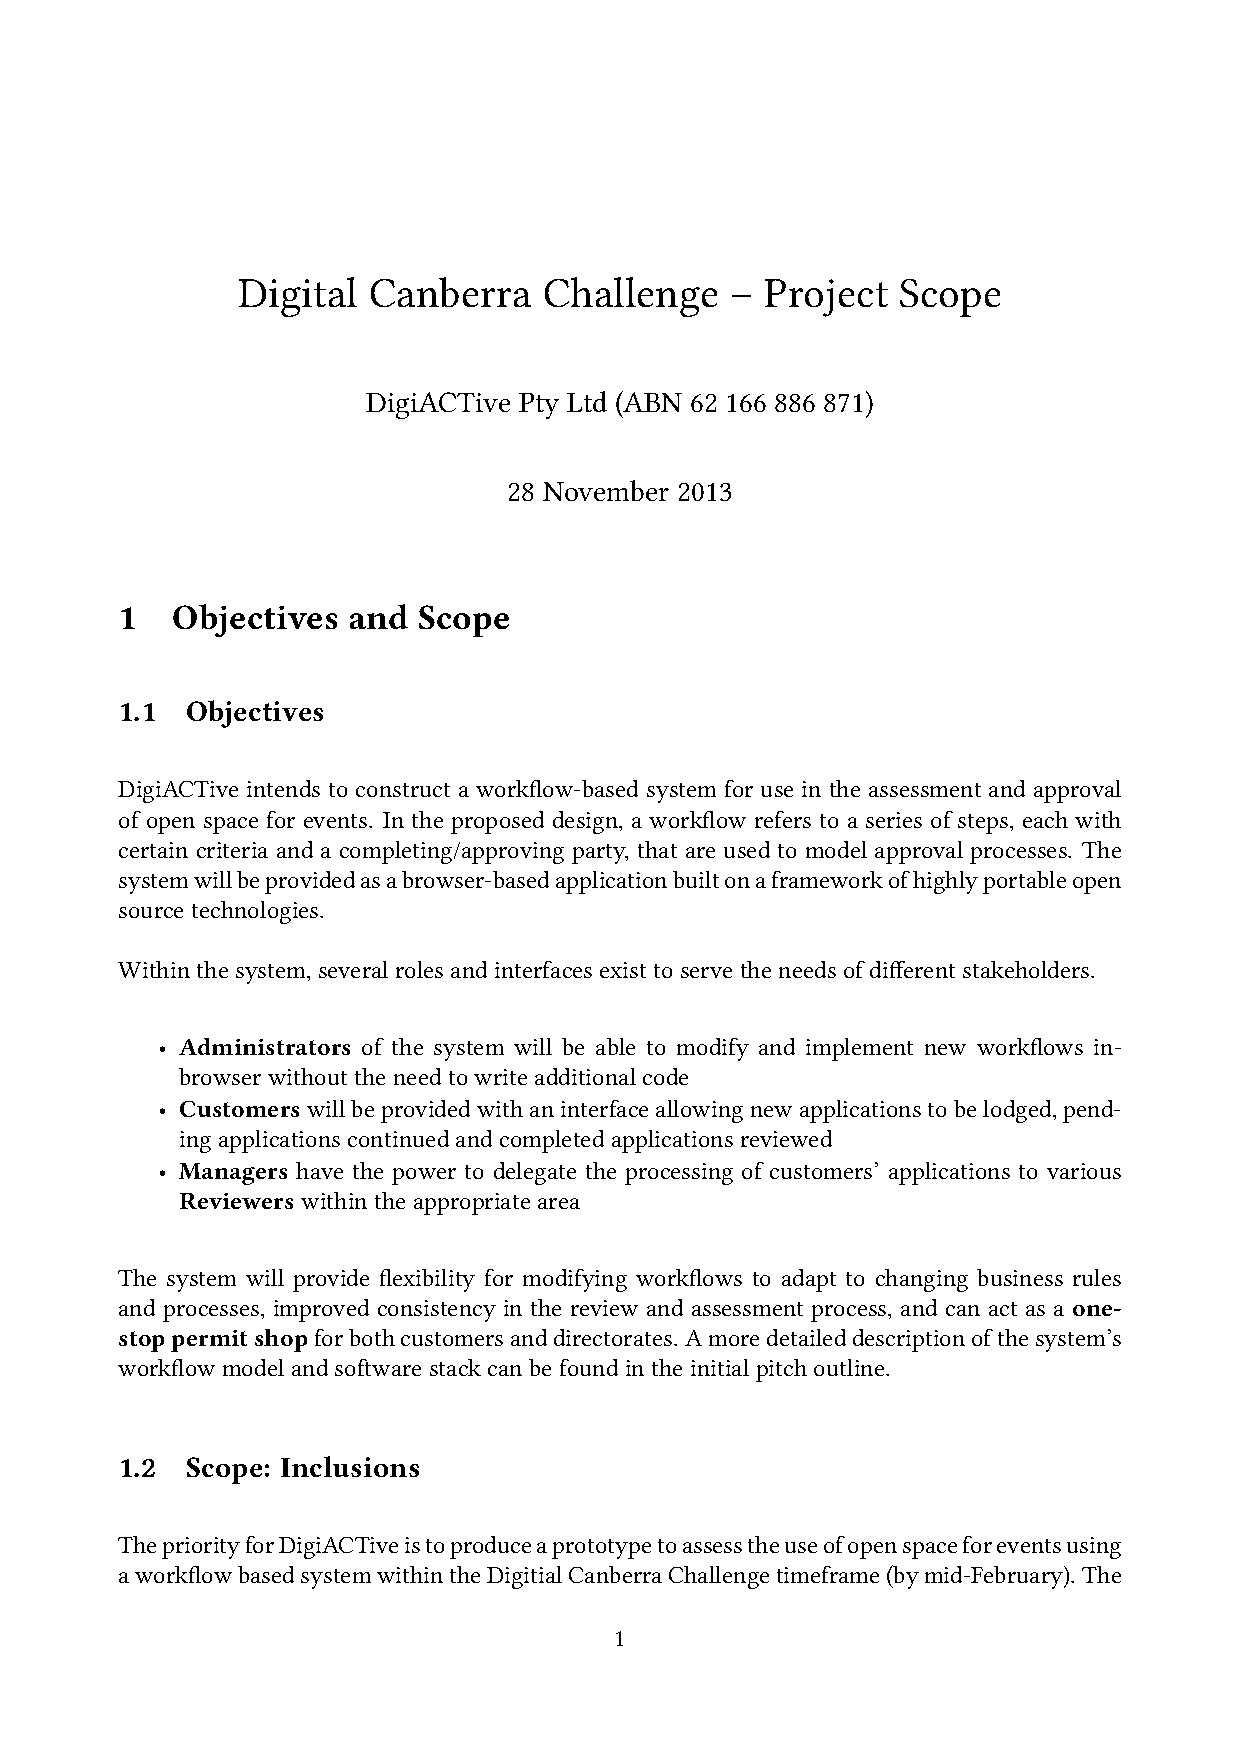
\includepdf[pages=1-6,nup=1x2,frame=true,landscape=true]{attached_work_scope.pdf}

\section{Attachment: Technical Brief}

This technical brief updates and extends the original pitch outline
available on the eGov Cluster shared folder.

The DigiApproval system considers the following ``characters'':

\begin{itemize}
\item
  An \emph{applicant} is someone trying to organise an event or apply
  for an approval.
\item
  There are one or more \emph{agencies} or \emph{directorates}.
\item
  There may be \emph{external stakeholders}.

  An \emph{agency} is a body that an applicant must work with to get one
  or more of the approvals they require. In this POC, all applications
  are initially made to TAMS/PACS, which is an agency.

  Within each agency, there are 3 roles:

  \begin{itemize}
  \itemsep1pt\parskip0pt\parsep0pt
  \item
    \emph{Administrators} are responsible for overseeing the system and
    setting up the application process as \emph{workflows} (detailed
    below).
  \item
    \emph{Approvers} work with applicants to progress their
    applications, applying their professional judgment and agency policy
    to determine when and how applications proceed to the next stage of
    the workflow.
  \item
    \emph{Managers} are responsible for allocating applications to
    approvers and ensuring that workload is balanced appropriately among
    approvers. (Future extensions may automate parts of this role, but
    are not in scope for the POC.)
  \end{itemize}

  As part of the application process, an applicant may also deal with
  other agencies:

  \begin{itemize}
  \itemsep1pt\parskip0pt\parsep0pt
  \item
    Applicanta may apply directly to other agencies for related types of
    approval. For example, INSERT EXAMPLE HERE
  \item
    If an application triggers appropriate predefined rules, the system
    can automatically send relevant parts (sub-workflows) of the
    application to other agencies for feedback and approval.
  \item
    Approvers may manually send part of the application to other
    agencies or external stakeholders for feedback and approval. (This
    is appropriate where automated rules cannot be developed and
    professional judgement is necessary.)
  \end{itemize}

  Agencies may be either \emph{in the system} or \emph{out of the
  system}.

  \begin{itemize}
  \itemsep1pt\parskip0pt\parsep0pt
  \item
    Agencies that are \emph{in the system} have their own
    administrators, approvers and managers -- they are handled entirely
    within the DigiApproval system.
  \item
    Agencies that are \emph{out of the system} have applications sent to
    them by email. Emails are sent through the DigiApproval web
    interface, and all emails are stored with the relevant application
    in a correspondence register.
  \end{itemize}

  This provides a way for the system to interoperate with agencies
  without them needing to take up the system internally.

  External stakeholders (e.g.~local businesses who may be affected by an
  event) are treated as if they are \emph{out of the system} agencies.
\end{itemize}

\subsection{User Interface}

The application will be a Web-based application, with both the applicant
front-end and the agency back-end accessible using a standard Web
browser, without any need for installing software on local computers.
The applicant front-end will be accessible from the wider Internet, with
the agency back-end accessible from approved ACT/Commonwealth Government
networks.

Based on our pitch, we see the user interface unfolding as follows.

\subsubsection{Applicants}

Before an applicant can begin a workflow, they must register as a user.

Once they register with their name and contact details, they will be
presented with a dashboard showing at a glance:

\begin{itemize}
\itemsep1pt\parskip0pt\parsep0pt
\item
  \textbf{Workflows that they can commence.} Once a workflow is
  commenced, the directorate is notified, and the application is
  assigned to an approver.
\item
  \textbf{Any existing applications that they have begun}, and the stage
  those applications are at. Applicants can pull up the details of their
  applications and see the entire history in one place. They can then
  make sure that they have completed any steps necessary for them to
  complete. The approver responsible for their application is notified
  whenever the applicant completes a step.
\item
  \textbf{A link to contact the approver assigned to help them progress
  their workflow}.
\item
  \textbf{A link to access previous completed applications}, should they
  need to re-download any documents/approvals, and to help them avoid
  duplicating effort if they arrange repeated events.
\end{itemize}

A very loose concept of what this might look like is below:

\begin{figure}[htbp]
\centering
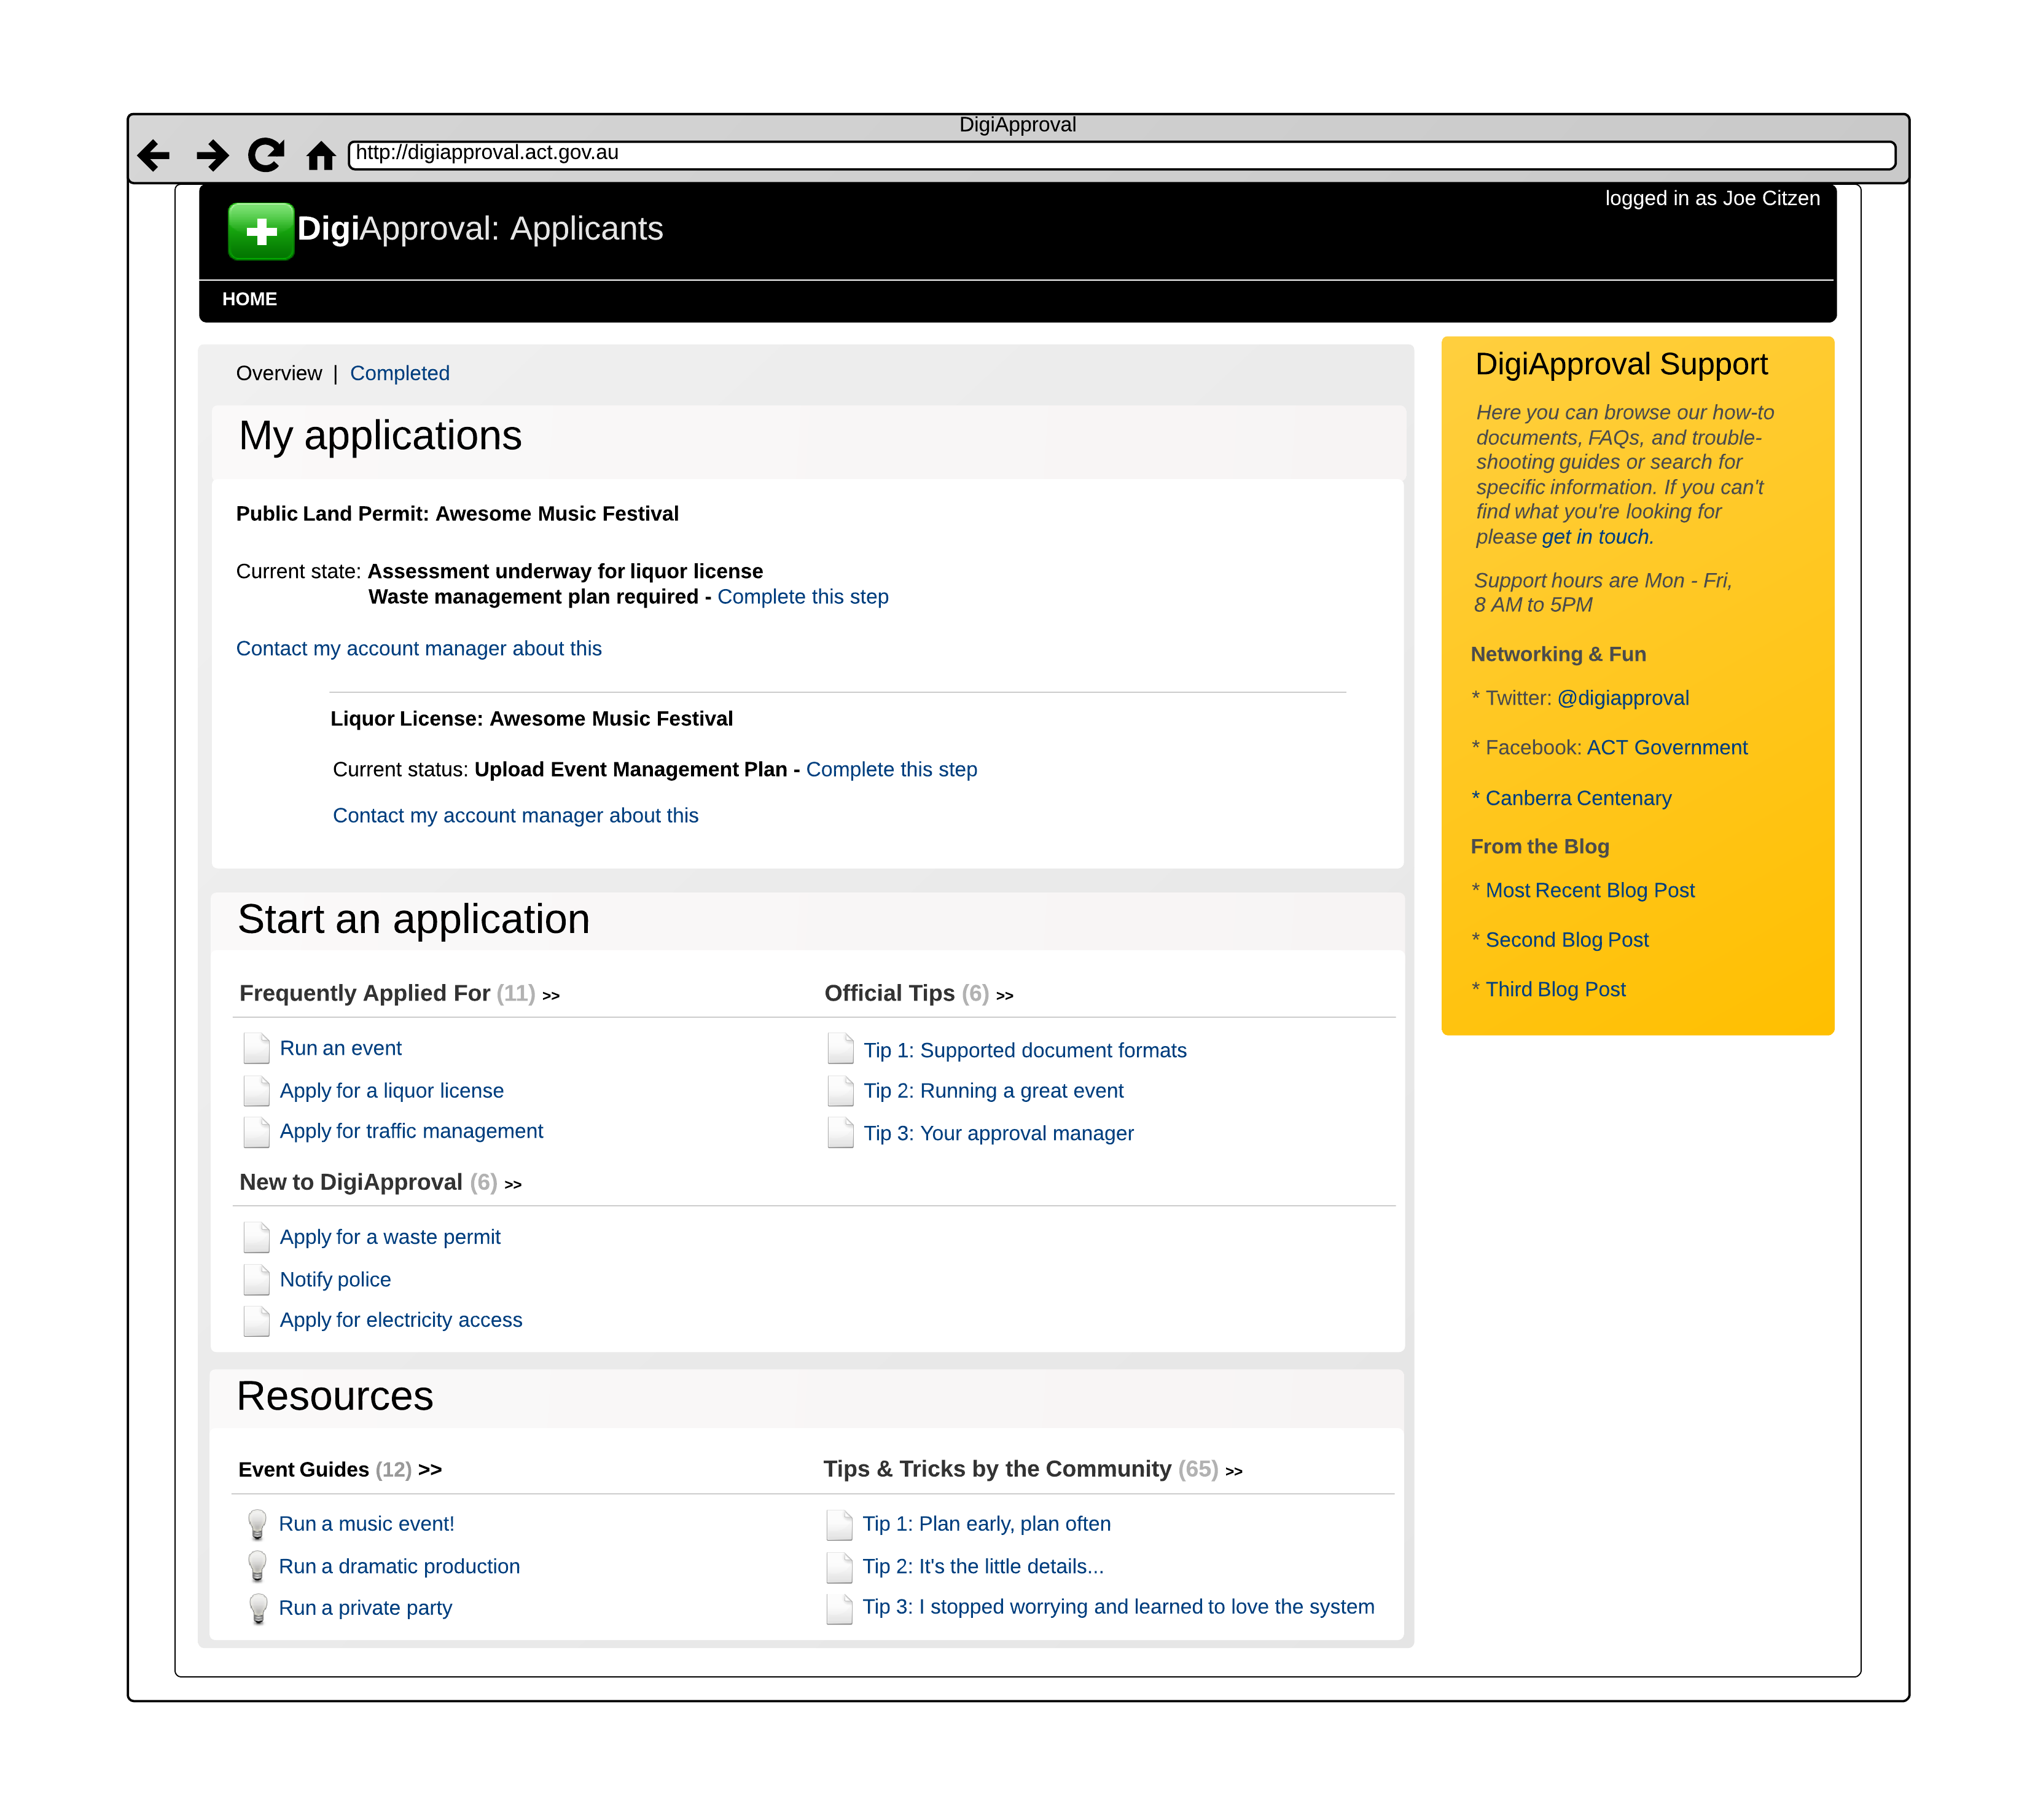
\includegraphics[width=0.9\textwidth]{./imgs/user-wireframe.png}
\caption{User wireframe}
\end{figure}

\subsubsection{Approvers}

When an approver logs in, they can see at a glance:

\begin{itemize}
\itemsep1pt\parskip0pt\parsep0pt
\item
  The applications for which they are responsible.
\item
  The status of those applications:

  \begin{itemize}
  \itemsep1pt\parskip0pt\parsep0pt
  \item
    Are they waiting on the applicant?
  \item
    Are they waiting on another agency? Is that agency responding
    promptly, or have they taken too long?
  \item
    Are they ``in my court''?
  \end{itemize}
\end{itemize}

Approvers can then pull up an application for which they are
responsible, see, in one place:

\begin{itemize}
\itemsep1pt\parskip0pt\parsep0pt
\item
  The entire history of the application
\item
  All the communications that have been exchanged
\item
  How long the application has been pending, both internally, and with
  any other agencies involved
\item
  Any steps necessary to progress it.
\end{itemize}

The applicant is notified whenever the approver completes a step, and
approvers (and possibly applicants) are notified when an involved agency
provides feedback.

A very loose concept of what this might look like is below. (This
concept sketch doesn't include the multi-agency amendments, but that is
in scope for the POC.)

\begin{figure}[htbp]
\centering
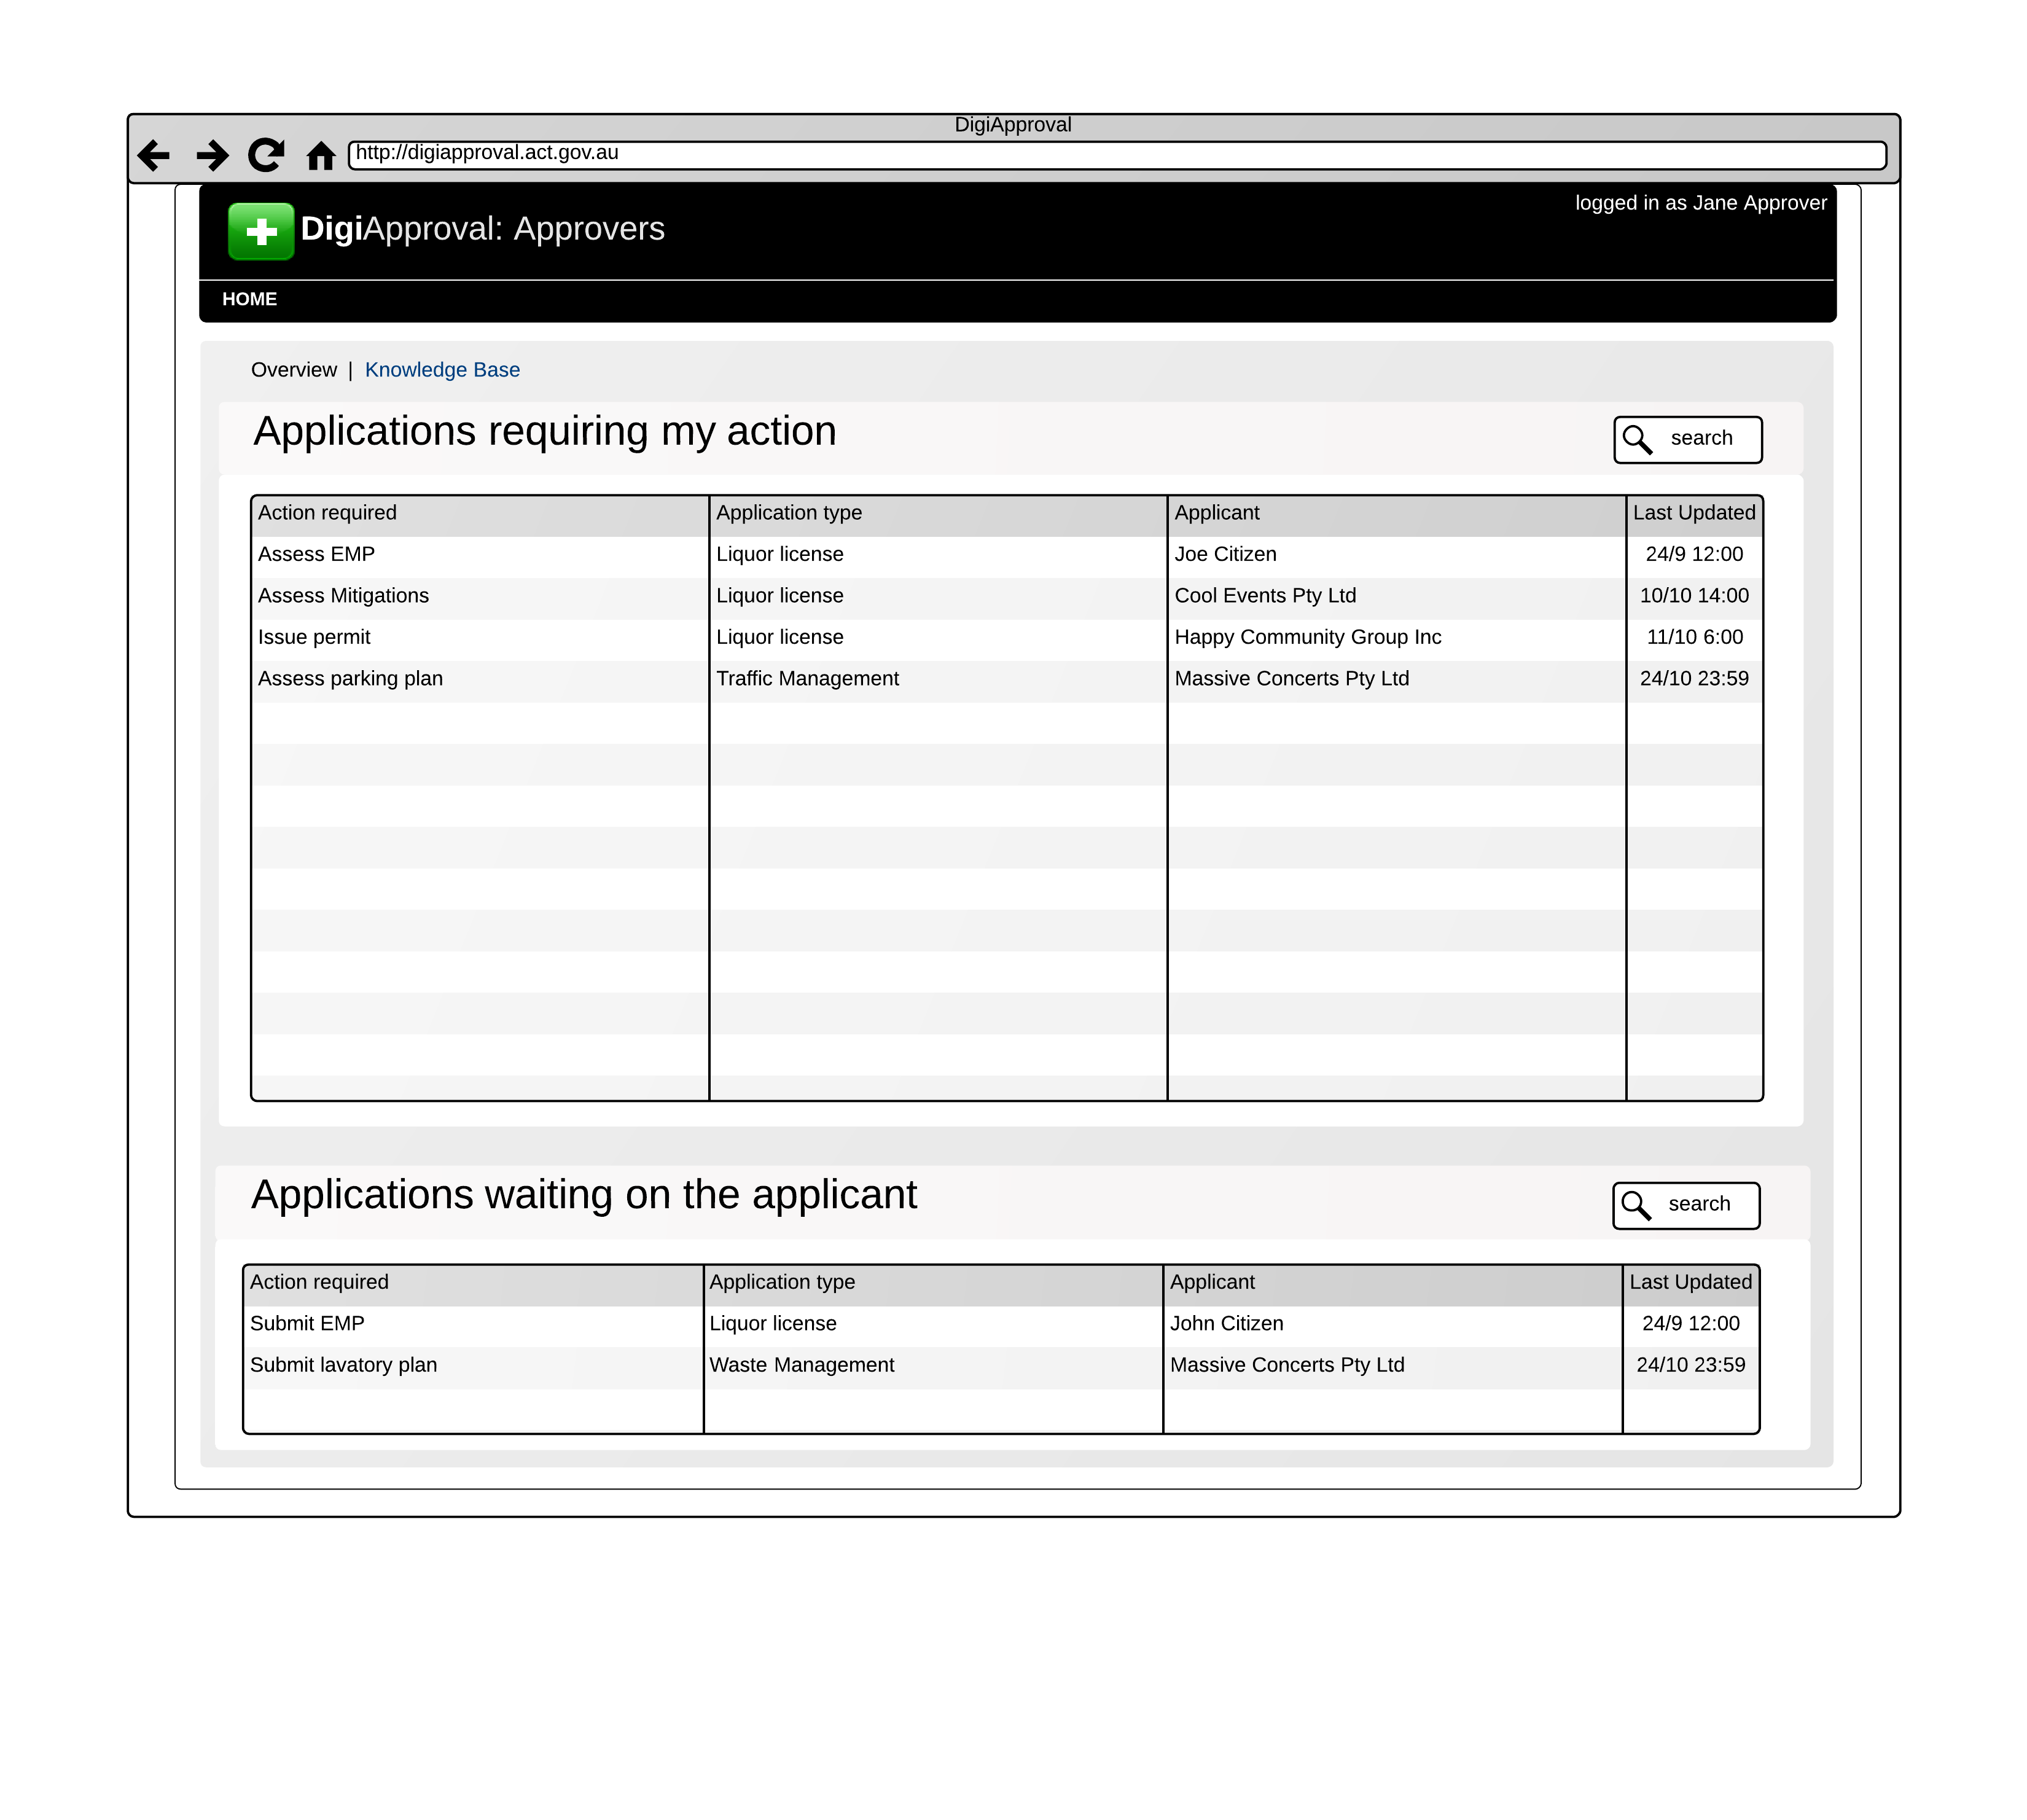
\includegraphics[width=0.9\textwidth]{./imgs/approver-wireframe.png}
\caption{Approver wireframe}
\end{figure}

\subsubsection{Managers}

A manager will have a simple user interface to assign a workflow that
has just commenced to an approver, and is able to re-allocate
in-progress workflows if needed. (For example, if an approver is ill or
leaves the directorate.)

Managers will also be able to generate reports, as follows.

\subsubsection{Reporting}

Based on stakeholder consultation, a reporting front-end has been added,
that can generate reports on (at a minimum):

\begin{itemize}
\itemsep1pt\parskip0pt\parsep0pt
\item
  A calendar basis: for a day, what approvals have been granted?
\item
  A location basis: for a location, what approvals have been granted?
\item
  A ``state'' basis: how many approvals are pending? How many have been
  granted/rejected recently? By whom?
\end{itemize}

All reports can be generated by managers and administrators. Some
reports (calendar/location) can be generated by approvers so as they do
not double-book events.

\subsection{Technology Stack}

Our solution can be decomposed into a web layer, an application layer, a
set of asynchronous workers and a storage layer (file store and
database).

\begin{figure}[htbp]
\centering
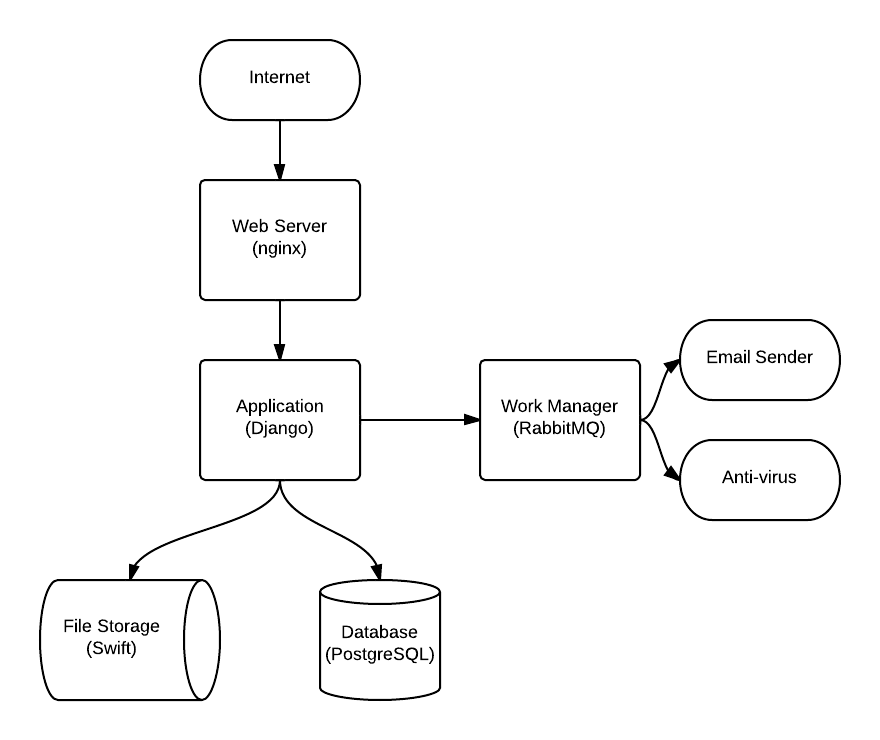
\includegraphics[width=0.9\textwidth]{./imgs/tech-overview.png}
\caption{Application architecture}
\end{figure}

Each of these layers is horizontally scalable.

The system will be implemented in \href{http://django.org}{Django}.
Django:

\begin{itemize}
\itemsep1pt\parskip0pt\parsep0pt
\item
  is a well known web framework for the Python programming language.
\item
  is used on sites that deal with millions of hits, so it is known to be
  able to scale.
\item
  has a large community of users. It will be easy to find Django
  developers capable of maintaining and extending the system.
\end{itemize}

The implementation focuses on scalability, security and portability to
SSICT systems. It is being built around:

\begin{itemize}
\itemsep1pt\parskip0pt\parsep0pt
\item
  \textbf{Operating System}: CentOS

  \begin{itemize}
  \itemsep1pt\parskip0pt\parsep0pt
  \item
    Largely equivalent to the RHEL environment prescribed by SSICT.
  \item
    Furthermore, our stack should also port without issue to Solaris, as
    preferred by SSICT.
  \end{itemize}
\item
  \textbf{Provisioning}: \href{http://www.opscode.com/chef/}{Chef},
  meeting the SSICT requirement for managed configuration over ad-hoc
  configuration.
\item
  \textbf{Web server}: \href{http://nginx.org/en}{nginx}, deploying SSL
  throughout.
\item
  \textbf{Application}: Django:

  \begin{itemize}
  \itemsep1pt\parskip0pt\parsep0pt
  \item
    Python 3.3 in preference to 2.7.
  \item
    A preference for using existing modules as opposed to developing our
    own functionality.
  \item
    The workflow engine is
    \href{https://github.com/knipknap/SpiffWorkflow}{SpiffWorkflow}.
  \end{itemize}
\item
  \textbf{Worker layer}: \href{http://rabbitmq.com}{RabbitMQ},
  interfaced through \href{http://www.celeryproject.org/}{Celery}.

  \begin{itemize}
  \itemsep1pt\parskip0pt\parsep0pt
  \item
    Virus scanning workers will be implemented in
    \href{http://www.clamav.net/lang/en/}{ClamAV}, or possibly stubbed
    out if we run out of time.
  \item
    Email workers will send mail through Amazon SES, using the SMTP
    interface for simple transition to SSICT infrastructure.
  \end{itemize}
\item
  \textbf{Database}: \href{http://postgresql.org}{PostgreSQL}.

  \begin{itemize}
  \itemsep1pt\parskip0pt\parsep0pt
  \item
    Transition to an Oracle database to meet SSICT requirements should
    be straightforward thanks to Django's database abstraction.
  \end{itemize}
\item
  \textbf{File storage}: \href{http://swift.openstack.org}{OpenStack
  Swift}.
\item
  \textbf{Front end}: \href{http://getbootstrap.com/}{Bootstrap} and
  \href{http://html5boilerplate.com/}{HTML5 boilerplate}

  \begin{itemize}
  \itemsep1pt\parskip0pt\parsep0pt
  \item
    Developed with an eye towards standards compliance, accessibility
    and extensibility.
  \end{itemize}
\end{itemize}

We will be developing our system on Amazon Web Services (AWS), however,
all the technologies have been chosen with a view to the code being
hosted on SSICT servers should the prototype proceed to a full system.

\subsubsection{Security}

Our system is designed to be able to solidly \emph{authenticate} users,
determine what those user are \emph{authorised} to do, ensure the
\emph{integrity} of their actions and the system as a whole, while
maintaining \emph{confidentially} of applicant and directorate
information, using industry best practices.

We will deploy SSL at the front end to ensure applicant passwords and
information is encrypted while in transit. We will be implementing as
much functionality as possible through standard libraries, reducing the
scope for security flaws and error on our part.

We will also be taking a proactive approach to security wherever
possible. For example, a major source of security flaws arise from not
verifying user input. Our system will make sure that we that user input
is valid, make sure that uploaded documents are of the expected format
and are free from known viruses, and so on, \emph{before} they are
presented to approvers.
\end{document}